\documentclass{fpgairpods}
\usepackage[letterpaper, margin=1in]{geometry}

\addbibresource{proposal.bib}
\graphicspath{{figs/}}

\setlist{noitemsep, topsep=0pt}

\begin{document}

{\Huge \textbf{FPGAirPods} Project Proposal}

\vspace{2mm}
{Gokul Kolady, Ben Kettle, Niko Ramirez | \today \ | 6.111}
\vspace{5mm}


\begin{multicols}{2}
\section{Overview}
Our 6.111 final project aims to implement active noise cancellation as seen in over-ear and in-ear headphones such as the Bose QC35 and the AirPods Pro (hence the name). In order to do this, we will first need to create a physical model of a single headphone (one ear cup) that we will use to test. Inside the ear cup, we will install a speaker (far from the ear) and a digital microphone (closer to the ear). We will also use a digital microphone external to the ear cup in order to capture ambient noise.

The FPGA itself will handle the computational side of the active noise cancellation. This will primarily involve an adaptive filter that will continually improve its coefficients in order to minimize the error function --- i.e., the noise that makes it through and is not cancelled out. We run the input from the external microphone through this filter, and play the filtered result out of the speaker with the aim of cancelling noise.

\section{Materials}


Several materials will be used in order to construct a prototype "headphone" to test on: 
\begin{itemize}
    \item 2x \href{https://www.adafruit.com/product/3421}{SPH0645LM4H microphone breakout boards} (\$7) from Adafruit will be used to collect noise from inside and outside the ear cup. These communicate via I2S, which will remove the need for ADCs between the microphone and the FPGA, and minimize potential for noise in the wires from the FPGA to the earpiece.
    \item 1x \href{https://www.adafruit.com/product/3968}{Speaker} (\$5) in order to play the anti-noise signal that we calculate into the user's ear. This is a 3W speaker, which should give adequate power. Another option is to use PC speakers that are powered by USB --- we could dissect these to remove one of the drivers, then build it into our cone. Either of these options will also need an amplifier such as the TPA2005-based USB boards available in the lab, as the onboard amp on the FPGA will not be able to drive this speaker.
    \item We will use a cup of some kind to mount all of these on.
    \item We'll create some passive noise insulation using some \href{https://www.amazon.com/Silverstone-21-Inch-Dampening-Acoustic-SF01/dp/B0040JHMH6?th=1}{foam} (\$20).
    \item We'll need some wire to connect the microphones and the speaker.
\end{itemize}

\end{multicols}


\begin{figure}[h]
\centering
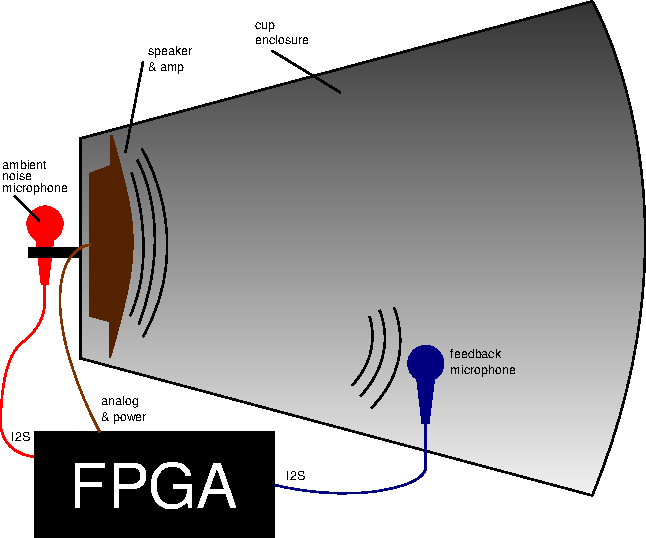
\includegraphics[width=300pt]{./figs/system_diagram_with_text.pdf}
\caption{The peripherals that will be included in our project}
\label{fig:peripherals}
\end{figure}

\begin{figure}
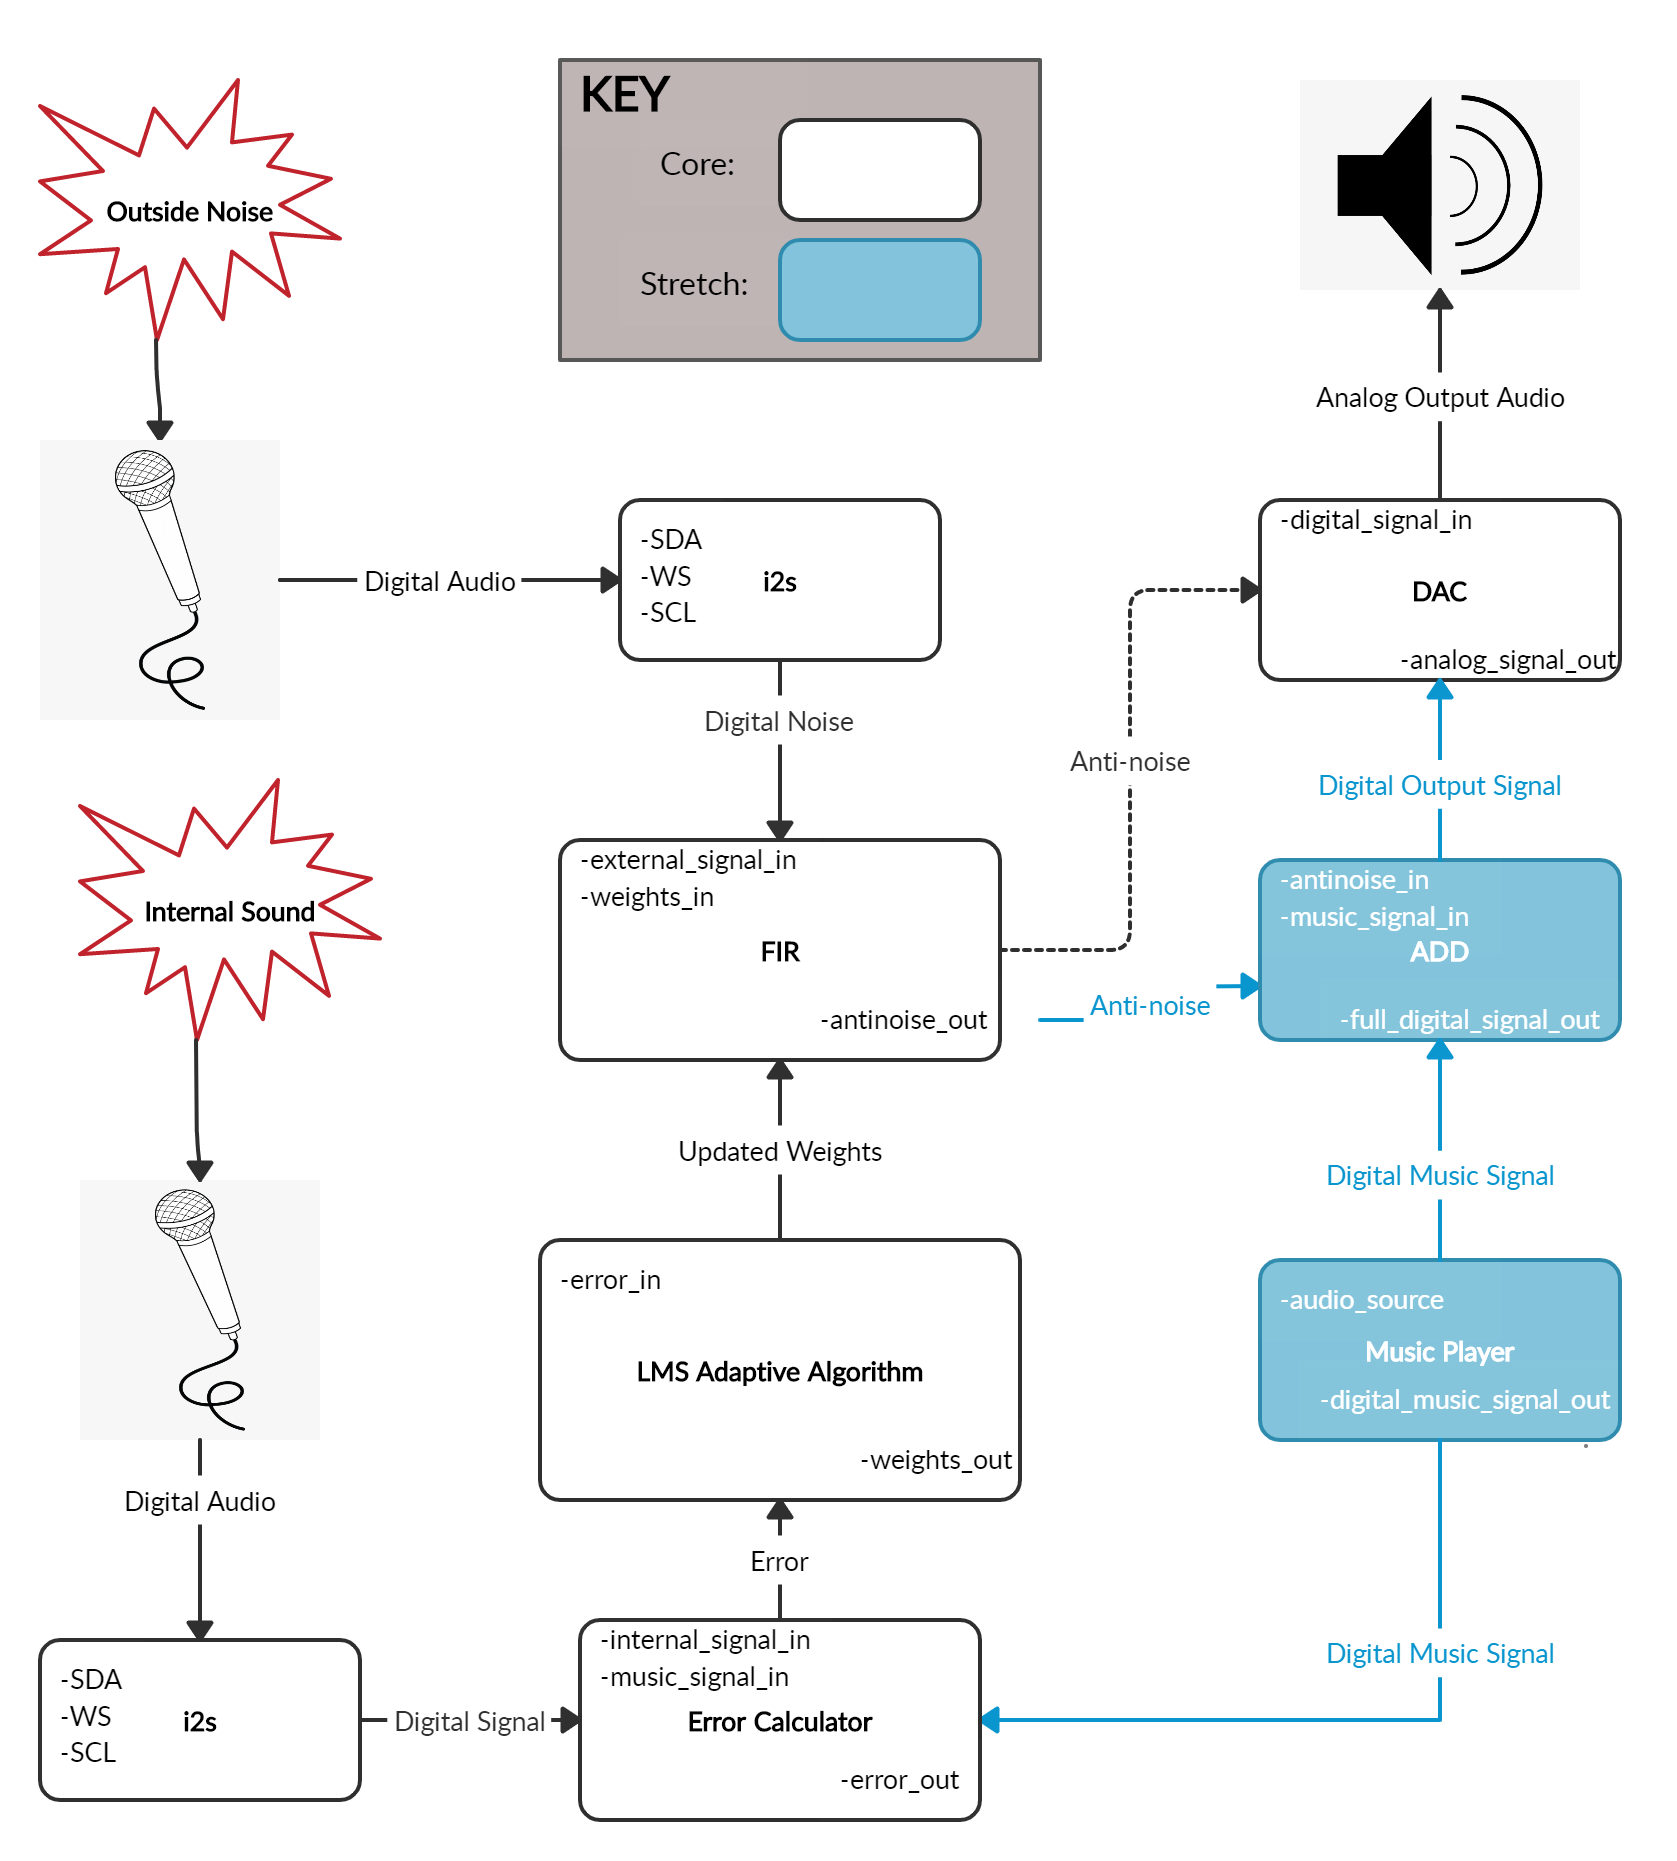
\includegraphics[width=\textwidth]{./figs/Proposal Block Diagram.png}
\caption{The high-level block diagram for our system.}
\label{fig:blockdiagram}
\end{figure}


\newpage
\begin{multicols*}{2}
\section{Modules}
\textbf{Note on Throughput:} In order to respond to incoming noise fast enough to cancel it out, we are aiming for a sampling rate of 100kHz throughout our system. Thus, with a 100MHz clock driving the FPGA, the computation that our system requires between samples must be completed within
\[ \frac{100\,000\,000}{100\,000} = 1000 \text{ clock cycles} \]
The full chain of modules will need to be completed in this time, but we anticipate many of them to complete in a single cycle---most of this will be used by the LMS algorithm to calculate the new weights, and the FIR filter to calculate the output for a given external noise input.

The core modules to be used in our final design are detailed below. Outside of these, we expect a number of modules to be created as part of the testing procedures.


\subsection{I2S Receiver - \textit{IP}}
This module will parse the incoming data stream from each of the two microphones. We can either implement it using the Vivado I2S IP, or implement it ourselves. We plan to implement it with IP initially, and if we are low on resources, we can look into implementing our own simpler version. There are several inputs and outputs associated with the AXI bus for the module, but the important ones include the core I2S signals and the resulting data. The IP I2S module outputs 32 bits, but we will then scale down to 16 bits due to the microphone's resolution (though we will test to make sure that its resolution is indeed limited to 16 bits as our research has suggested). 
\subsubsection{Inputs}
\begin{itemize}
    \item \ttt{SDA} - Microphone Data
    \item \ttt{WS} - Word Select
    \item \ttt{SCL} - Audio Clock
\end{itemize}
\subsubsection{Outputs}
\begin{itemize}
    \item \ttt{m_axis_aud_tdata[31:0]}: the primary output data --- in this case, a single sample from the microphone.
\end{itemize}
\subsubsection{Complexity/Level of Performance}
Because this is an IP module, its resource usage is clearly given in Vivado's documentation.
\begin{itemize}
    \item 476 LUTs
    \item 1722 FFs
    \item 1 36k BRAM
\end{itemize}

\subsection{FIR Filter - \textit{Niko}}
The FIR Filter module convolves the external ambient noise with a set of filter coefficients in order to produce an anti-noise signal. This anti-noise signal is later used to cancel out the ambient noise that makes it into the ear cup. These coefficients are set continuously by the LMS adaptive algorithm module.
\subsubsection{Inputs}
\begin{itemize}
    \item \ttt{external_signal_in[15:0]}: The current sample from the external microphone that will be filtered.
    \item \ttt{weights_in[31:0][9:0]}: Coefficients that the filter will use for convolution.
\end{itemize}
\subsubsection{Outputs}
\begin{itemize}
    \item \ttt{antinoise_out[15:0]}: Anti-noise signal that will be used to cancel out ambient noise.
\end{itemize}
\subsubsection{Complexity/Level of Performance}
This module will be time sensitive, as we will want to calculate the output corresponding to a given input in very little time in order to enable effective noise cancellation. Because of this, we anticipate a significant amount of time to be spent streamlining the functionality of the filter module and improving its performance. As part of this, we need fast access to the previous samples to use for the convolution, so these previous samples from the external microphone will be stored in a circular buffer as a 32 element array with each element 16 bits wide. Implementing this as a BRAM would be to slow, so it will be implemented with distributed RAM. Some optimization that we are considering for this module is performing the additions in a tree structure rather than sequentially and streamlining the multiplications if necessary. We expect this to include 32 multiplications and 32 additions.

\subsubsection{Testing - \textit{Gokul}}
Testing for this module will consist of simple inputs similar to those seen in Lab 5a with known filter coefficients, such as a low pass filter with an impulse input, a sine input, etc. If these show the results that we expect, we can conclude that the FIR filter works. Later, we will also test it in conjunction with the LMS.

\subsection{LMS Adaptive Alg. - \textit{Ben \& Gokul}}
This module uses the LMS adaptive algorithm in order to update the coefficients of the FIR Filter for better noise cancellation. This algorithm takes advantage of the steepest descent optimization method, which analyzes the impact of the previous filter coefficients on the observed error and computes appropriate adjustments. This update is accomplished using the following equation\cite{lmsfilter}, where $b_k(n)$ is the FIR coefficient for a given $k$ value and a given timestep $n$, $\Lambda$ is a predefined step size or learning rate that defines how quickly the filter weights change, $e(n)$ is the calculated error, $f(n)$ is the value of the noise sample from the external microphone at a timestep $n$, and $M$ is the number of coefficients in the FIR filter:
\[ b_k(n + 1) = b_k(n) + \Lambda e(n)f(n-k) \]
\[ k = 0, 1, 2,\ldots,  M-1 \]

\subsubsection{Inputs}
\begin{itemize}
    \item \ttt{external_signal_in[15:0]}: The current sample from the external microphone (previous samples get used in weight update formula, so they must be stored in this module).
    \item \ttt{error_in[15:0]}: The error between the internal microphone signal and the desired signal.
\end{itemize}
\subsubsection{Outputs}
\begin{itemize}
    \item \ttt{weights_out[31:0][9:0]}: Updated coefficients to be used by the FIR filter in the next timestep for improved anti-noise generation.
\end{itemize}
\subsubsection{Complexity/Level of Performance}
To implement this operation, we will need to store the last $M$ noise inputs from the external microphone along with the full last set of filter coefficients. Previous samples from the external microphone will be stored in a circular buffer as a 32 element array each 16 bits wide, and the coefficients will be stored similarly in distributed RAM if possible, 32 elements each 10 bits wide.

\subsubsection{Testing - \textit{Niko}}
Testing this module will be a bit more involved than some of the others due to its not well-defined behavior, but in order to test the behavior we will need to have a working FIR module. With this module in place, we can then test the ability of the LMS algorithm to recreate the coefficients of a given filter. In other words, we can have our "desired" signal be the result of passing some input through an arbitrary filter, use this desired signal to calculate the error $e(n)$, and pass this error into our LMS module. If the input of the LMS module is the same as the input to this mystery filter, we can conclude that the LMS algorithm is functioning as necessary.

\subsection{Error Calculator - \textit{Ben}}
The error calculator computes the difference between the output of the internal microphone (the sound within the ear cup) and the intended final audio. If we reach our stretch goal, the intended audio will be the music being inputted into the system. Otherwise, the goal will be silence. This difference or "error" will be fed into the LMS module for error correction.
\subsubsection{Inputs}
\begin{itemize}
    \item \ttt{internal_signal_in[15:0]}: The current sample from the internal microphone that will be used for error calculation.
    \item \ttt{music_signal_in[15:0]}: The internal microphone signal will be compared to this signal for error calculation (this signal will be input music if we reach our stretch goal, and silence otherwise).
\end{itemize}
\subsubsection{Outputs}
\begin{itemize}
    \item \ttt{error_out[15:0]}: The difference between the internal microphone's signal and the desired signal.
\end{itemize}
\subsubsection{Complexity/Level of Performance}
The module requires no sophisticated storage or optimization, as it only involves a singular subtraction. 


\subsection{DAC - \textit{Gokul}}
The DAC (Digital-to-Analog Converter) module will be used to transform the final digital output audio into a PWM signal to be passed to the amplifier onboard the FPGA. This is fairly simple, and has been mostly done in lab. No significant resources are required.
\subsubsection{Inputs}
\begin{itemize}
    \item \ttt{digital_signal_in[15:0]}: The digital signal to be converted.
\end{itemize}
\subsubsection{Outputs}
\begin{itemize}
    \item \ttt{analog_signal_out}: The PWM output to the amplifier.
\end{itemize}
\subsubsection{Testing - \textit{Ben}}
Testing will consist of verifying that the correct PWM duty cycle is outputted for a given known input, and later by feeding simple signals such as a sine wave into the module and ensuring that the speaker outputs the correct audio.

\subsection{Music Player - \textit{Gokul}}
This stretch goal module outputs the source music/audio from a connected device (such as a phone over aux) in digital form (the user should ideally hear a version of this audio with minimal corruption). With the possible extension of Bluetooth-based input audio, this module would be modified to take its input from a Bluetooth module that would be interfaced with the FPGA.
\subsubsection{Inputs}
\begin{itemize}
    \item \ttt{audio_input[15:0]}: The digital output from the XADC.
    \item \ttt{enable}: whether the music should be played.
\end{itemize}
\subsubsection{Outputs}
\begin{itemize}
    \item \ttt{digital_music_signal_out[15:0]}: The digital music signal from the module's audio source. 
\end{itemize}
\subsubsection{Complexity/Level of Performance}
In order to do this, we will need to use the onboard XADC to read the audio that the user is inputting, either via an aux cord or via an attached Bluetooth module. Because the XADC provides us with digital data, we only need to change the bit width to match the 16 bits used elsewhere if necessary. This aspect would be fairly simple, and would require no arithmetic. 
\subsubsection{Testing - \textit{Ben}}
Testing this module would first involve testing the XADC itself, and verifying that our setup for connecting an external device to the system works properly. We also need to verify that for a given input voltage to the XADC, the output sample that we expect is the result.

\subsection{Add - \textit{Niko}}
If we reach our stretch goal of the music player integration, we will need a module to merge the output of the FIR --- the signal that will cancel the incoming noise --- with the music to play. This module will take two signals as an input, and output their sum. It will be very simple, and require no internal memory. The only complexity here will be to ensure that the sum does not roll over beyond the limits of the bit width.
\subsubsection{Inputs}
\begin{itemize}
    \item \ttt{antinoise_in[15:0]}: One of the two signals to be added.
    \item \ttt{music_signal_in[15:0]}: The other signal to be added.
\end{itemize}
\subsubsection{Outputs}
\begin{itemize}
    \item \ttt{full_digital_signal_out[15:0]}: The sum of the two signals.
\end{itemize}



\section{Stretch Goal}

\subsection{Playable Music}
Primary stretch goal as mentioned above in depth in the modules section under \textit{Music Player} and \textit{Add}. The primary goal is to use an aux cord in order to play the music. The secondary goal beyond an aux cord would be implementing Bluetooth to play the music. 

\section{Cool Extensions}
\textbf{*In no particular order, and only if time permits}

\subsection{Implementing Physical Headphones}
Instead of using a cup to model our noise-canceling headphones, we can modify a real pair of headphones. This would require disassembling the headphones, attaching a microphone inside, attaching a microphone outside, and using two FPGAs to handle the left and right headphone.

\subsection{Select-able Hard-coded Songs}
Allow the user of the headphones to select between a given number of songs that are stored on the FPGA. This would require the use of additional memory (perhaps BRAM) in order to hold a small database of music.


\subsection{Transparency Mode}
This would aim to achieve the opposite purpose of the noise cancelling, working to counteract the acoustic muffling of the case with the goal of sounding as though there is no headphone being worn at all. This would involve the same LMS algorithm, but would change the error function.

\subsection{Toggle Keyword Recognition}
Use microphone input to recognize when someone near the user speaks the user's name and switch to transparency mode. The idea is that when someone needs the user's attention, the headphone intelligently switches to transparency mode to allow the user to clearly hear their surroundings.

\section{References}
\vspace{-7mm}
\printbibliography

\end{multicols*}


\end{document}
